\documentclass[class=NCU_thesis, crop=false]{standalone}
\usepackage[newfloat]{minted}
\usepackage{floatrow}
\usepackage{graphicx}


\begin{document}

\chapter{實驗設計與結果}

\section{實驗一:機械臂的基本控制}
\subsection{機械結構設計圖}
本實驗的硬體部分使用了3D列印技術,結合小型伺服馬達,設計了一個頂端為夾爪的小型機械臂,以下為此設備的詳細設計圖紙:
\begin{figure}[htbp]
    \centering
    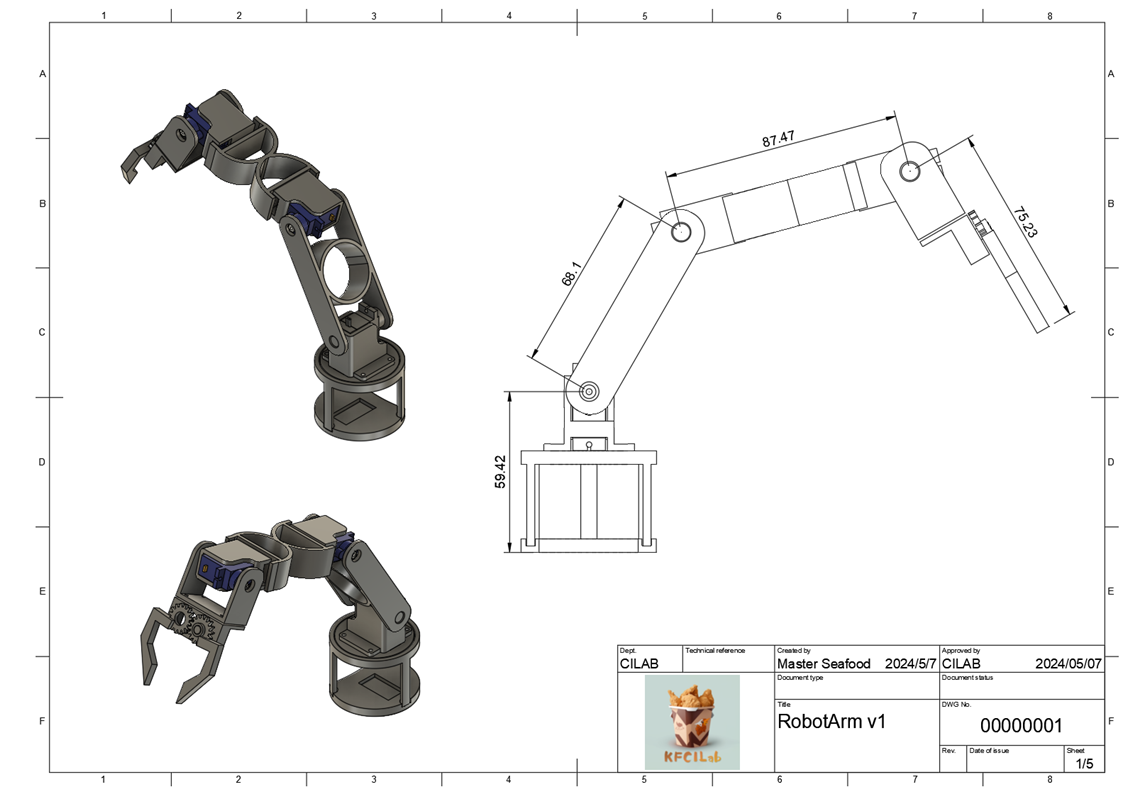
\includegraphics[width=0.9\textwidth]{figures/Armv1 (1).PNG}
    \caption{實驗一:設計圖紙 第一頁(單位:mm)}
    %\label{fig:Armv1Drawing_p1}}
\end{figure}

\begin{figure}[htbp]
    \centering
    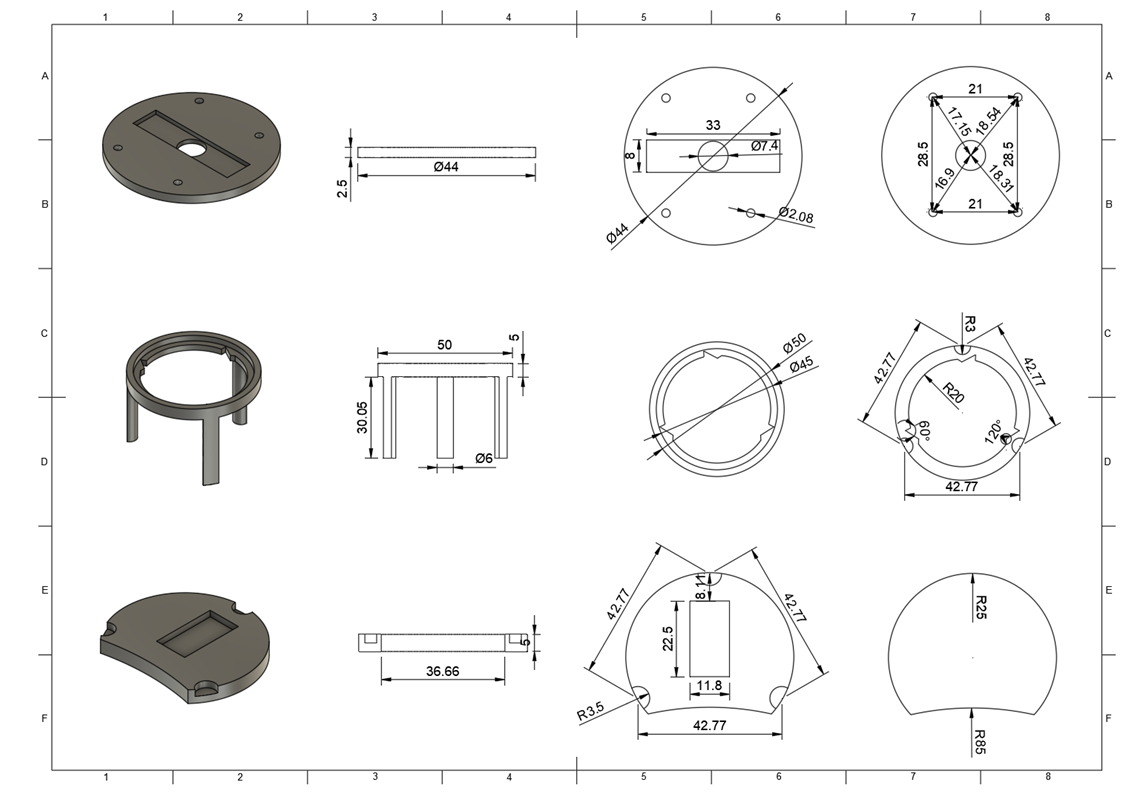
\includegraphics[width=0.9\textwidth]{figures/Armv1 (2).PNG}
    \caption{實驗一:設計圖紙 第二頁(單位:mm)}
\end{figure}

\begin{figure}[htbp]
    \centering
    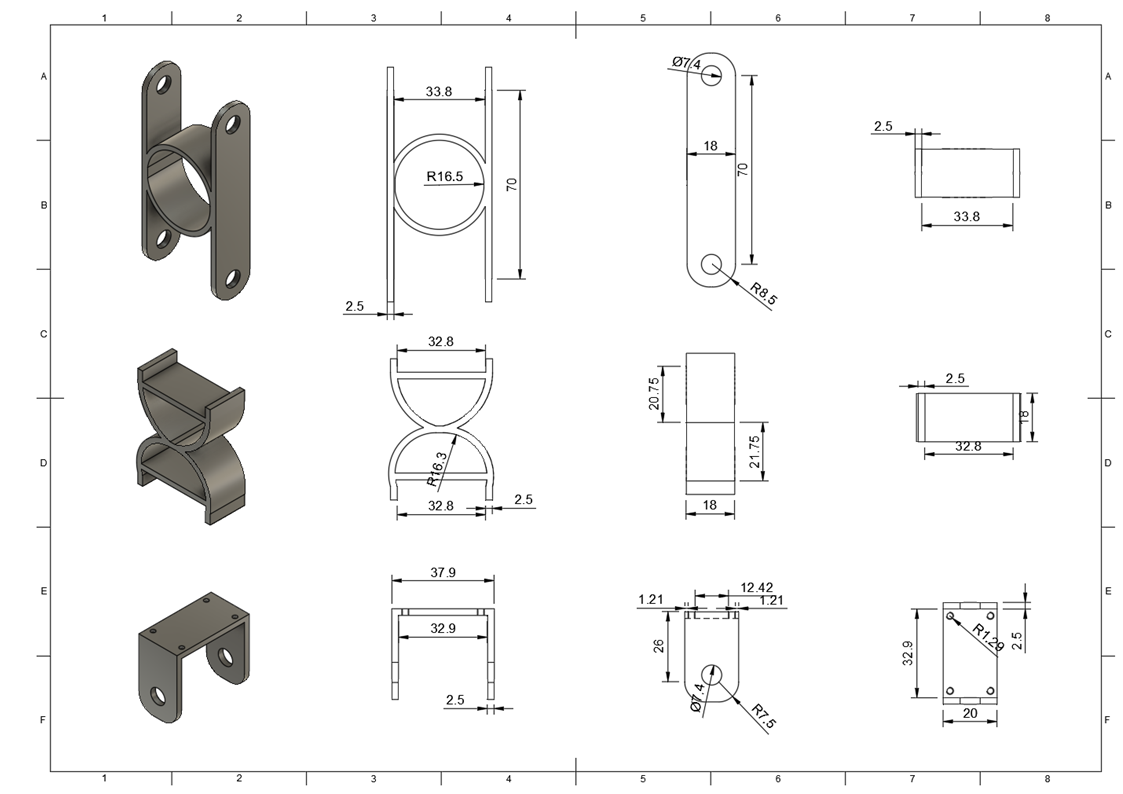
\includegraphics[width=0.9\textwidth]{figures/Armv1 (3).PNG}
    \caption{實驗一:設計圖紙 第三頁(單位:mm)}
\end{figure}

\begin{figure}[htbp]
    \centering
    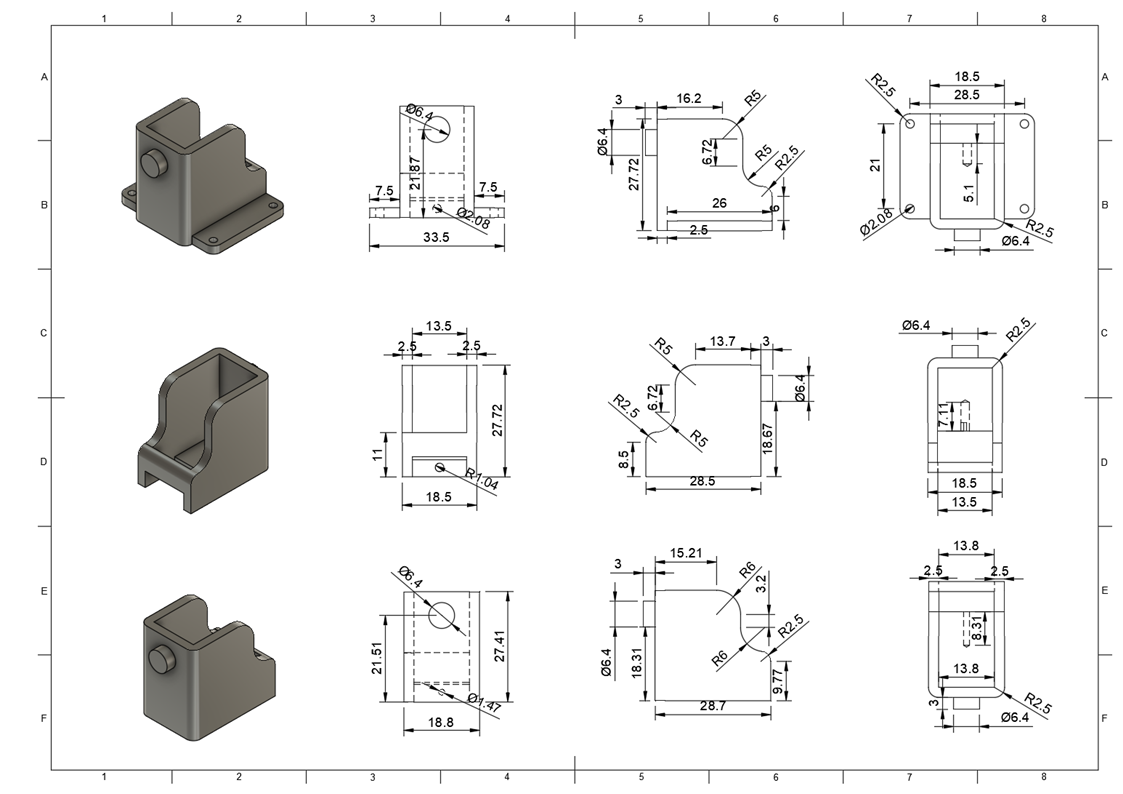
\includegraphics[width=0.9\textwidth]{figures/Armv1 (4).PNG}
    \caption{實驗一:設計圖紙 第四頁(單位:mm)}
\end{figure}

\begin{figure}[htbp]
    \centering
    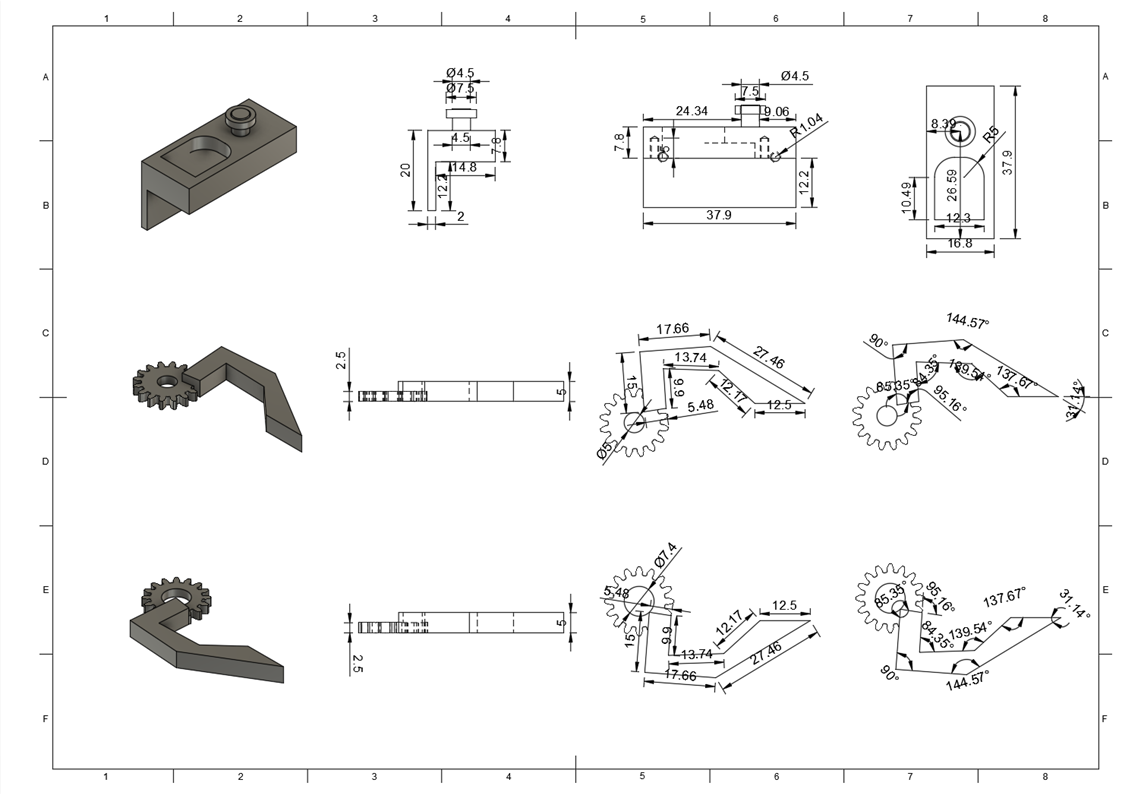
\includegraphics[width=0.9\textwidth]{figures/Armv1 (5).PNG}
    \caption{實驗一:設計圖紙 第五頁(單位:mm)}
\end{figure}

\subsection{函數設計}
在這個實驗中,我們的目標是讓機械臂能夠成功夾取特定物體,並放置於指定位置。
這個過程涉及機械臂路徑的規劃和精確的抓取動作。
為了實現這一目標,我們撰寫了一個簡易的路徑規劃程式,
利用語言模型在填空方面的優勢,使其生成和編輯機械臂的運動指令。
使用這樣的方式,嘗試讓大型語言模型自動生成適當的路徑規劃,並將其應用於機械臂的控制,
以下為此實驗使用的程式碼:\\
\begin{listing}[h]
    \begin{minted}[frame=single,
                   framesep=3mm,
                   linenos=true,
                   xleftmargin=21pt,
                   tabsize=4]{python}
        from ArmEnv_3D_ori import ArmEnv_3D
        import math

        Arm = ArmEnv_3D([5.942, 6.81, 8.747, 7.523], False)
        path = []
        #Please planning path form hear
        #path+=Arm.moveto([0, 0, 25], 20) explain: Move to [0, 0, 25] in 20 steps
        #path+=[[-91, 0, 0, 0]] explain: Close claw
        #path+=[[91, 0, 0, 0]] explain: Open claw

        #reset
        end=path[-2].copy()
        while not sum(end)==0:
            for i in range(len(end)):
                if end[i]>0: end[i]-=1
                elif end[i]<0: end[i]+=1
            path.append(end.copy())
    \end{minted}
\caption{實驗程式碼} 
\end{listing}
\clearpage

\subsection{下達指令的格式範例}
\begin{listing}[h]
    \begin{minted}[frame=single,
                   framesep=3mm,
                   linenos=true,
                   xleftmargin=21pt,
                   tabsize=4]{js}
    {     
        role: "user",
        content : 
    "\
    from ArmEnv_3D_ori import ArmEnv_3D\
    import math\
    \
    Arm = ArmEnv_3D([5.942, 6.81, 8.747, 7.523], False)\
    path = []\
    #Please planning path form hear\
    #path+=Arm.moveto([0, 0, 25], 20) explain: Move to [0, 0, 25] in 20 steps\
    #path+=[[-91, 0, 0, 0]] explain: Close claw\
    #path+=[[91, 0, 0, 0]] explain: Open claw\
    \
    #reset\
    end=path[-2].copy()\
    while not sum(end)==0:\
        for i in range(len(end)):\
            if end[i]>0: end[i]-=1\
            elif end[i]<0: end[i]+=1\
        path.append(end.copy())\
    "
    },
    {
        role: "user", 
        content: "This is a sample program for controlling a robotic arm.\
                  Please modify it to help me complete the following requirements: \
                  the ball is at [10.5, 12, 2], and the top of the tower is at [9.5, 0, 14.5]. \
                  Please help me catch the ball to the top of the tower. \
                  During the process, please do not get too close to the side of the tower \
                  (keep outside the radius 7).\
                  return only code.\
                  "
    }
    \end{minted}
\caption{實驗一:指令格式範例} 
\end{listing}

\begin{listing}[h]
    \begin{minted}[frame=single,
                   framesep=3mm,
                   linenos=true,
                   xleftmargin=21pt,
                   tabsize=4]{js}

    {
        role="assistant",
        content=
    "\
    from ArmEnv_3D_ori import ArmEnv_3D\
    import math\
    \
    Arm = ArmEnv_3D([5.942, 6.81, 8.747, 7.523], False)\
    path = []\
    path += Arm.moveto([0, 0, 25], 20)\
    path += Arm.moveto([10.5, 12, 2], 20)\
    path+=[[-91, 0, 0, 0]]\
    path += Arm.moveto([10, 13, 15], 20)\
    path += Arm.moveto([9.5, 0, 14.5], 20)\
    path+=[[91, 0, 0, 0]]\
    \
    #reset\
    end=path[-2].copy()\
    while not sum(end)==0:\
        for i in range(len(end)):\
            if end[i]>0: end[i]-=1\
            elif end[i]<0: end[i]+=1\
        path.append(end.copy())\
    "
    }

    \end{minted}
\caption{實驗一:回傳格式範例} 
\end{listing}
\clearpage

\subsection{實驗結果}
以下為本實驗的實驗過程縮圖與總結:\\

\begin{table}[h]
    \centering
    \caption{實驗結果:Please catch the ball to the top of the tower.}
    \begin{tabular}{ccccc}
    \hline
    大型語言模型 & 總次數 & 成功次數 & 失敗次數 & 成功率 \\
    \hline
    GPT-4o & 10 & 7 & 3 & 0.7\\
    \hline
    GPT-3.5 Turbo & 10 & 4 & 6 & 0.4\\
    \hline
    \end{tabular}
\end{table}

根據本實驗結果顯示,使用大型語言模型進行路徑規劃的效果相當不錯,並且隨著語言模型技術的發展,路徑規劃的準確率也有顯著的提升。然而,目前的方法需要將整個程式碼放入語言模型的輸入中以生成控制程式碼,這種方式過於繁瑣。此外,這種方法也需要提供大量的前置條件,使用起來相當不便。因此,我們認為有必要對這個實驗進行進一步的調整,以提高其實用性和效率。

\clearpage
\begin{figure}[h]
    \centering
    \subcaptionbox
        {初始位置
        \label{fig:fig-dataset-contrast-after-adjustment}}
        {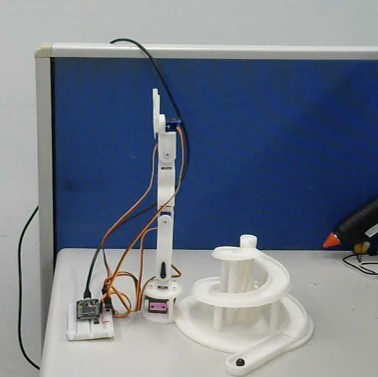
\includegraphics[width=0.4\linewidth]{figures/TB (1).jpg}}
    ~    
    \subcaptionbox
        {移動至黑球位置
        \label{fig:fig-dataset-contrast-after-adjustment}}
        {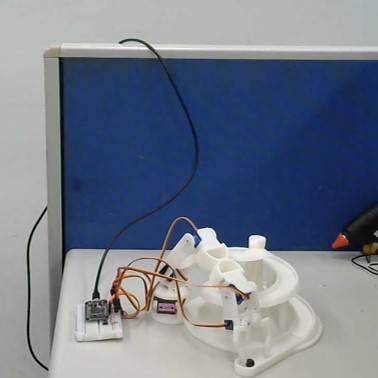
\includegraphics[width=0.4\linewidth]{figures/TB (2).jpg}}
    ~
    \subcaptionbox
        {夾取黑球
        \label{fig:fig-dataset-contrast-after-adjustment}}
        {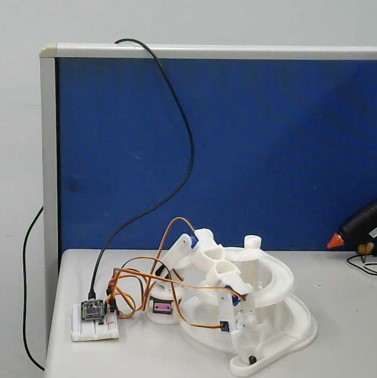
\includegraphics[width=0.4\linewidth]{figures/TB (3).jpg}}
    ~
    \subcaptionbox
        {移動至塔頂位置
        \label{fig:fig-dataset-contrast-after-adjustment}}
        {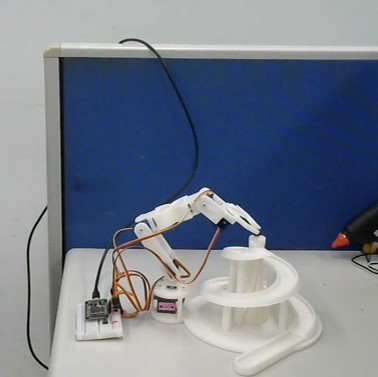
\includegraphics[width=0.4\linewidth]{figures/TB (4).jpg}}
    ~    
    \subcaptionbox
        {放開黑球
        \label{fig:fig-dataset-contrast-after-adjustment}}
        {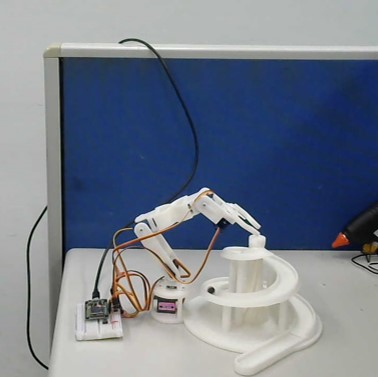
\includegraphics[width=0.4\linewidth]{figures/TB (5).jpg}}
    ~
    \subcaptionbox
        {回到初始位置
        \label{fig:fig-dataset-contrast-after-adjustment}}
        {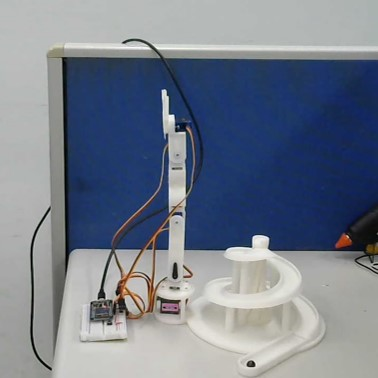
\includegraphics[width=0.4\linewidth]{figures/TB (6).jpg}}   
\caption{實驗一:實驗過程縮圖}
\end{figure}

\section{實驗二:將機械臂用於畫圖}
\subsection{機械結構設計圖}
本實驗的硬體部分使用了3D列印技術,結合小型伺服馬達,
設計了一個可夾取畫筆的小型機械臂,以下為此設備的詳細設計圖紙:
\begin{figure}[htbp]
    \centering
    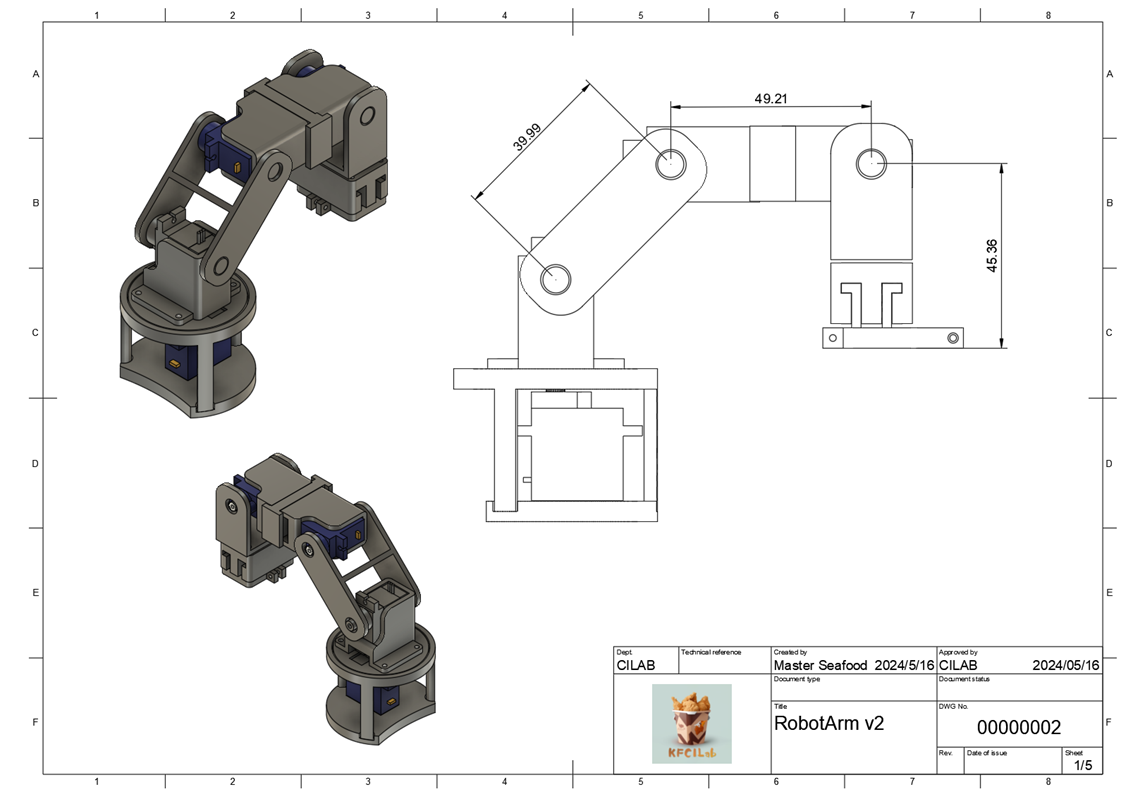
\includegraphics[width=0.9\textwidth]{figures/Armv2 (1).PNG}
    \caption{實驗二:設計圖紙 第一頁(單位:mm)}
    %\label{fig:Armv1Drawing_p1}}
\end{figure}

\begin{figure}[htbp]
    \centering
    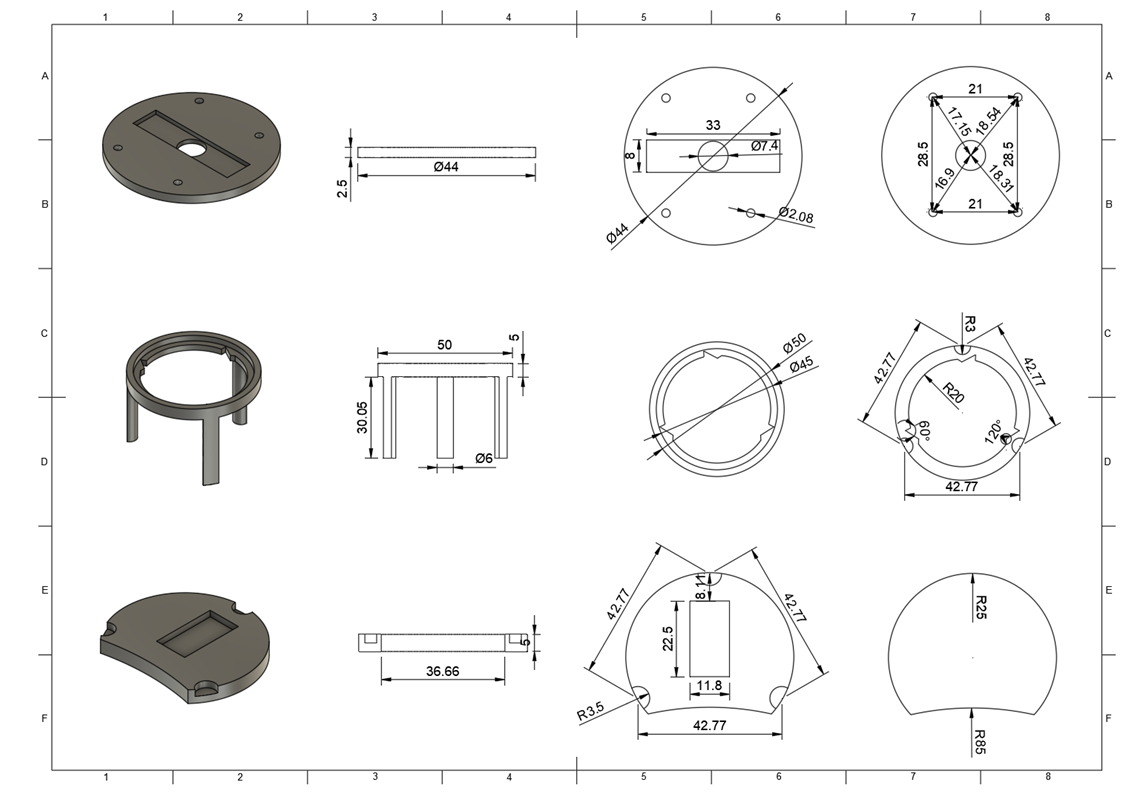
\includegraphics[width=0.9\textwidth]{figures/Armv2 (2).PNG}
    \caption{實驗二:設計圖紙 第二頁(單位:mm)}
\end{figure}

\begin{figure}[htbp]
    \centering
    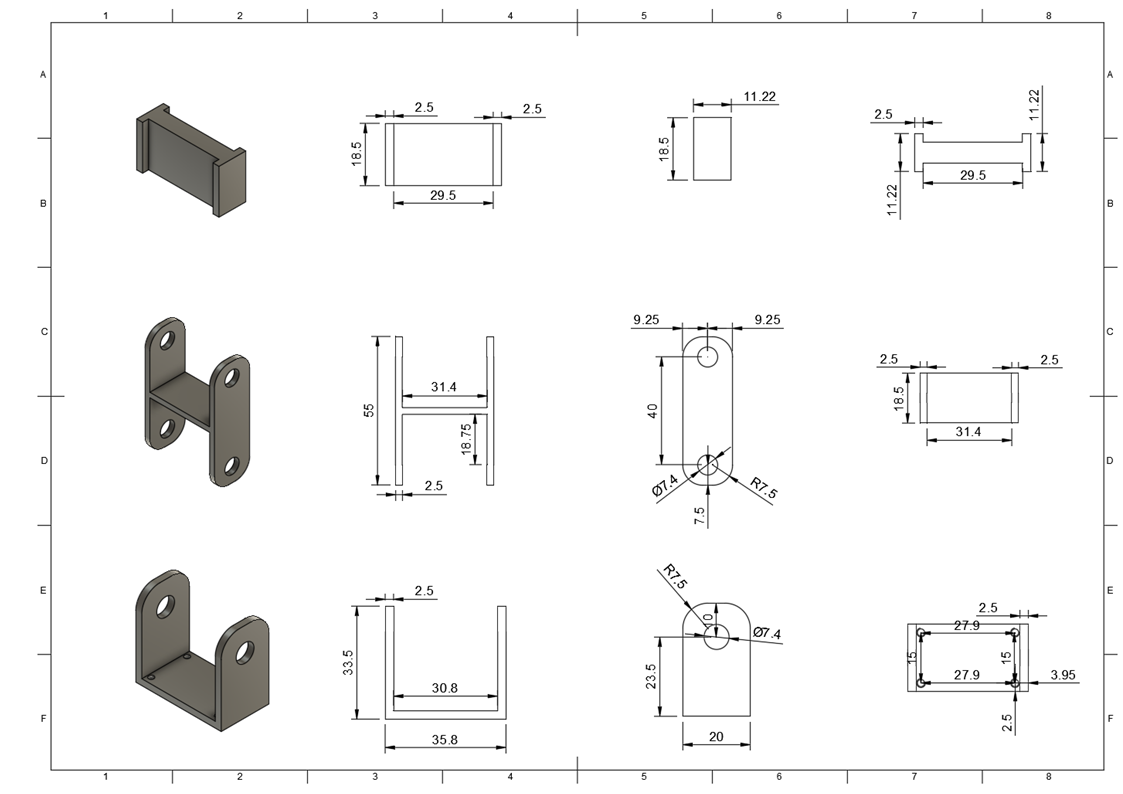
\includegraphics[width=0.9\textwidth]{figures/Armv2 (3).PNG}
    \caption{實驗二:設計圖紙 第三頁(單位:mm)}
\end{figure}

\begin{figure}[htbp]
    \centering
    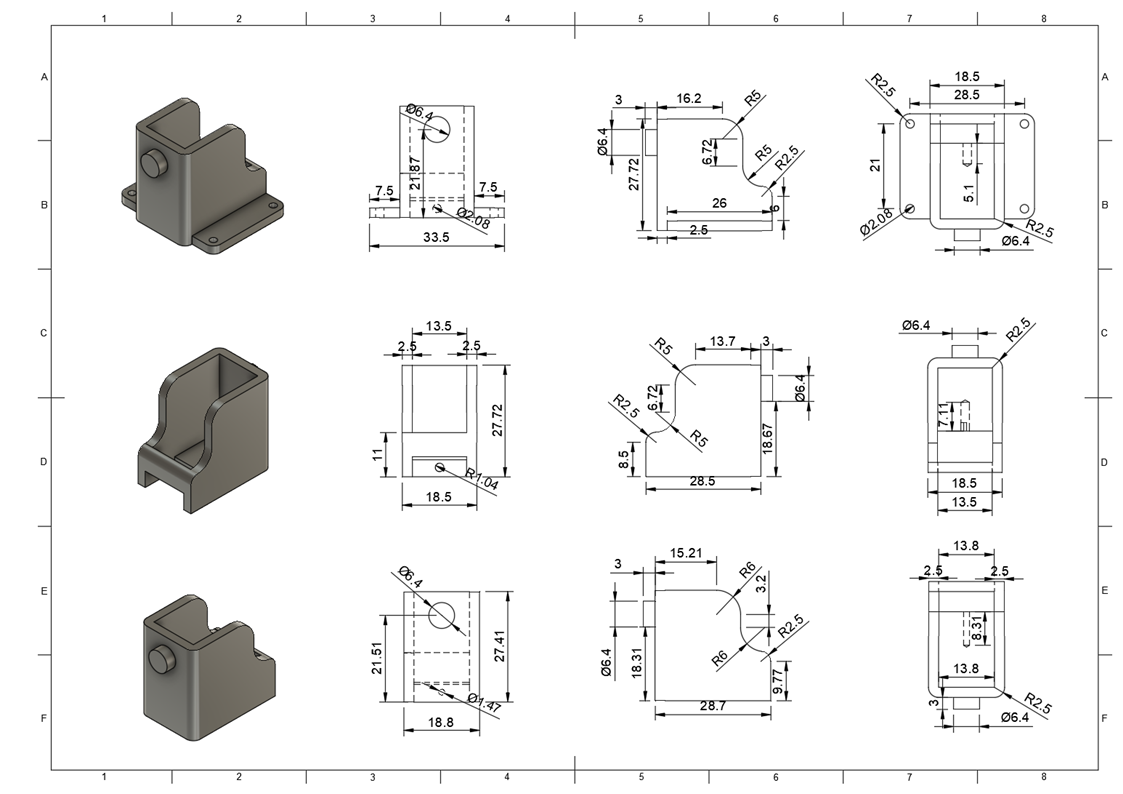
\includegraphics[width=0.9\textwidth]{figures/Armv2 (4).PNG}
    \caption{實驗二:設計圖紙 第四頁(單位:mm)}
\end{figure}

\begin{figure}[htbp]
    \centering
    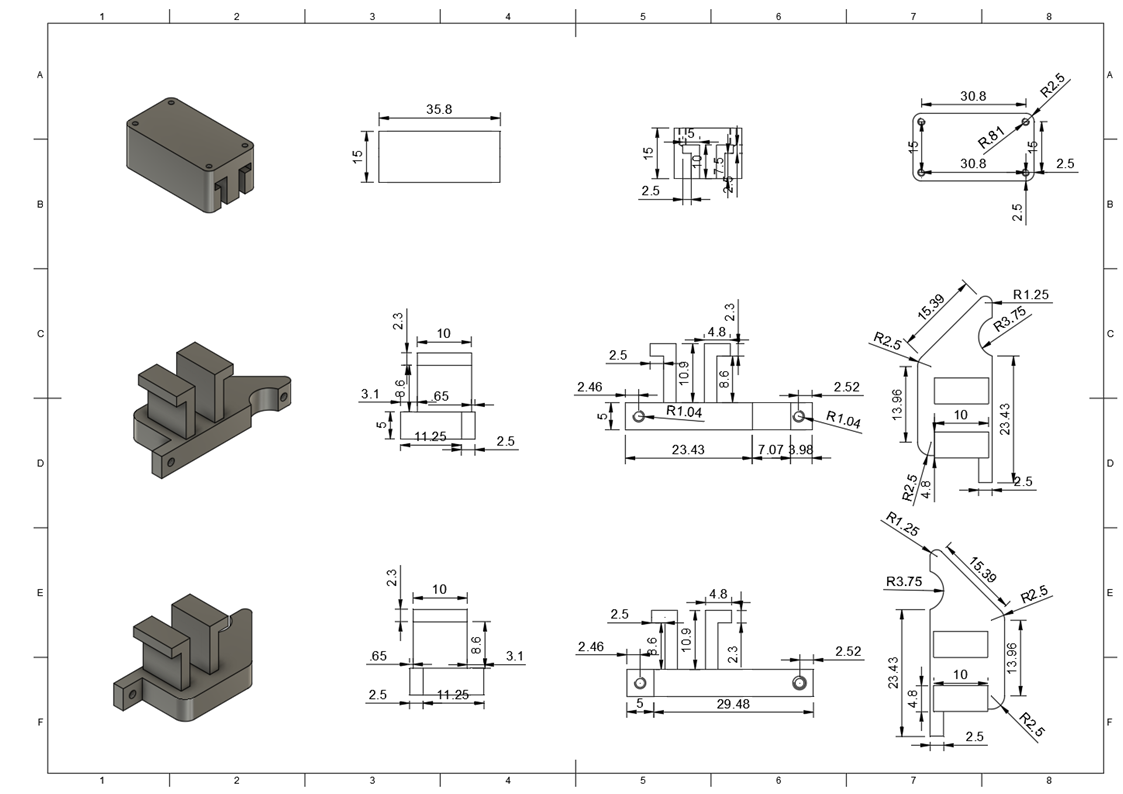
\includegraphics[width=0.9\textwidth]{figures/Armv2 (5).PNG}
    \caption{實驗二:設計圖紙 第五頁(單位:mm)}
\end{figure}

\subsection{函數設計}
從實驗一的基礎上,我們改進了機械臂的路徑規劃方法,將其應用於讓機械臂進行畫畫。
此次實驗中,我們簡化了路徑規劃,使大型語言模型在平面座標內進行規劃,
這樣可以降低複雜度,並節省資源。通過這種簡化的路徑規劃方法,
我們能夠更有效地控制機械臂,讓其能夠在紙上或畫布上繪製出預定的圖案。
本實驗將此機器的動作指令簡化為以下函式:

\begin{itemize}
    \item draw(from, to): 由變數from提供的座標,畫至變數to提供的座標。
\end{itemize}
\clearpage
\subsection{下達指令的格式範例}
\begin{listing}[h]
    \begin{minted}[frame=single,
                   framesep=3mm,
                   linenos=true,
                   xleftmargin=21pt,
                   tabsize=4]{js}
    {     
        role: "user",
        content : 
        "The following functions are available:\
        \
        draw(from, to): Let the arm draw a straight line from from to to,\
        such as draw([0, 0], [5, 5]).\
        the limit is[0, 5]\
        \
        Please help me use the above functions to control the robot arm,\
        and do not output other text other than the above functions.\
        (Use "," to separate each step)"
    },
    {
        role: "user", 
        content: "Task: Draw a square."
    }
    \end{minted}
\caption{實驗二:指令格式範例} 
\end{listing}

\begin{listing}[h]
    \begin{minted}[frame=single,
                   framesep=3mm,
                   linenos=true,
                   xleftmargin=21pt,
                   tabsize=4]{js}

    {
        role="assistant",
        content="draw([1, 1], [1, 4]),\
                 draw([1, 4], [4, 4]),\
                 draw([4, 4], [4, 1]),\
                 draw([4, 1], [1, 1])"
    }

    \end{minted}
\caption{實驗二:回傳格式範例} 
\end{listing}

\clearpage
\subsection{實驗結果}

以下為本實驗的實驗過程縮圖與總結:\\

\begin{table}[h]
    \centering
    \caption{實驗結果:Draw a square.}
    \begin{tabular}{ccccc}
    \hline
    大型語言模型 & 總次數 & 成功次數 & 失敗次數 & 成功率 \\
    \hline
    GPT-4o & 10 & 10 & 0 & 1\\
    \hline
    GPT-3.5 Turbo & 10 & 10 & 0 & 1\\
    \hline
    \end{tabular}
\end{table}

\begin{table}[h]
    \centering
    \caption{實驗結果:Draw a triangle.}
    \begin{tabular}{ccccc}
    \hline
    大型語言模型 & 總次數 & 成功次數 & 失敗次數 & 成功率 \\
    \hline
    GPT-4o & 10 & 10 & 0 & 1\\
    \hline
    GPT-3.5 Turbo & 10 & 10 & 0 & 1\\
    \hline
    \end{tabular}
\end{table}

\begin{table}[h]
    \centering
    \caption{實驗結果:Draw a star.}
    \begin{tabular}{ccccc}
    \hline
    大型語言模型 & 總次數 & 成功次數 & 失敗次數 & 成功率 \\
    \hline
    GPT-4o & 10 & 9 & 1 & 0.9\\
    \hline
    GPT-3.5 Turbo & 10 & 5 & 5 & 0.5\\
    \hline
    \end{tabular}
\end{table}

% \begin{table}[h]
%     \centering
%     \caption{實驗結果:Draw a house.}
%     \begin{tabular}{ccccc}
%     \hline
%     大型語言模型 & 總次數 & 成功次數 & 失敗次數 & 成功率 \\
%     \hline
%     GPT-4o & 10 & 7 & 3 & 0.7\\
%     \hline
%     GPT-3.5 Turbo & 10 & 0 & 10 & 0\\
%     \hline
%     \end{tabular}
% \end{table}

在這次實驗中,我們針對上一個實驗中存在的問題進行了改進。首先,我們將複雜的三維空間路徑規劃簡化為平面路徑規劃。使整個控制系統不再需要提供冗長的程式碼與相關條件,只需提供特定的圖形,就能驅動機械臂進行繪圖的控制模式,從實驗結果可以看出,這種改進的控制方式不僅大大減少了輸入和回傳的資料量,同時也保持了相當不錯的準確率。這表明此簡化方法在實現高效控制的同時,並未犧牲其性能。因此,我們決定將實驗繼續沿著這個方向進行調整和優化。

\clearpage
\begin{figure}[h]
    \centering
    \subcaptionbox
        {執行畫方形指令
        \label{fig:fig-dataset-contrast-after-adjustment}}
        {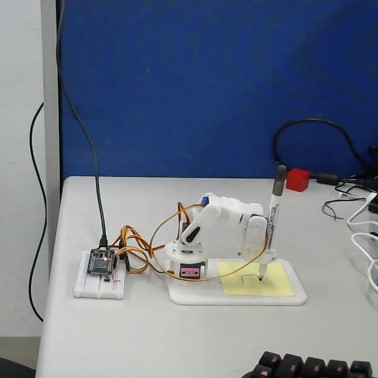
\includegraphics[width=0.4\linewidth]{figures/square_0.jpg}}
    ~    
    \subcaptionbox
        {完成畫方形指令
        \label{fig:fig-dataset-contrast-after-adjustment}}
        {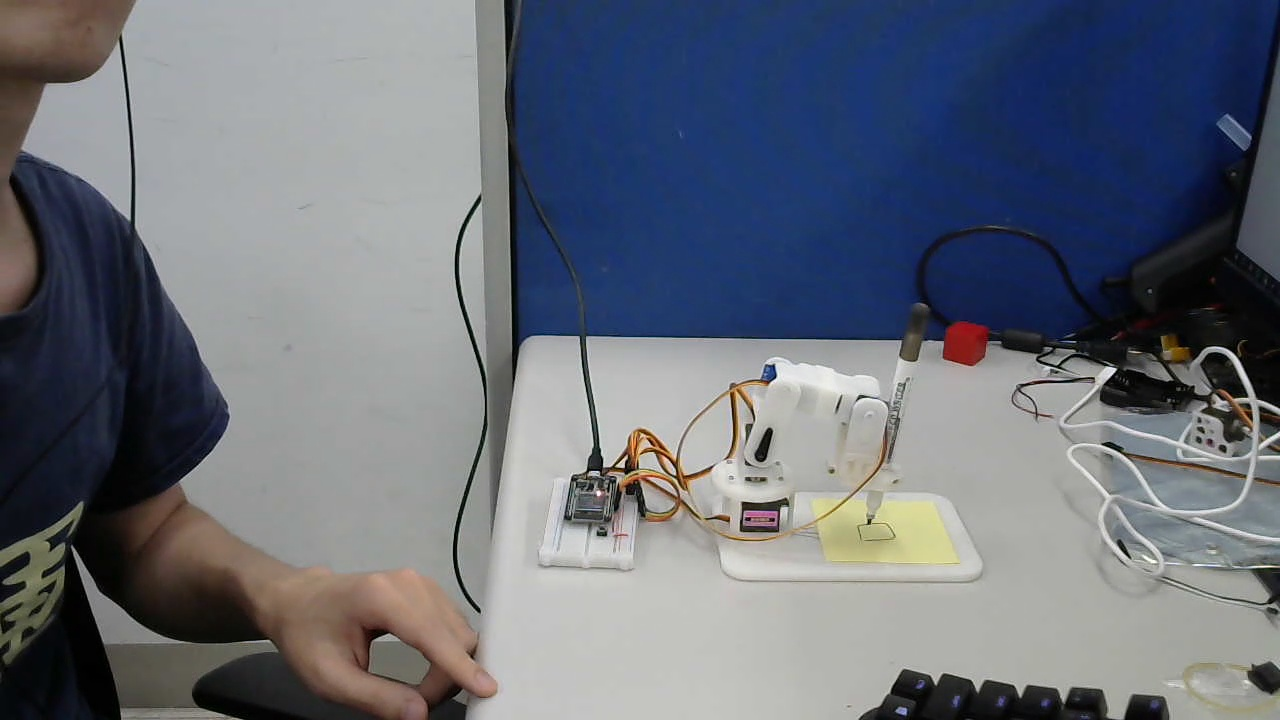
\includegraphics[width=0.4\linewidth]{figures/square_1.jpg}}
    ~
    \subcaptionbox
        {執行畫三角形指令
        \label{fig:fig-dataset-contrast-after-adjustment}}
        {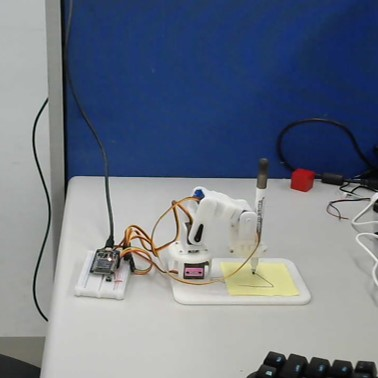
\includegraphics[width=0.4\linewidth]{figures/triangle_0.jpg}}
    ~
    \subcaptionbox
        {完成畫三角形指令
        \label{fig:fig-dataset-contrast-after-adjustment}}
        {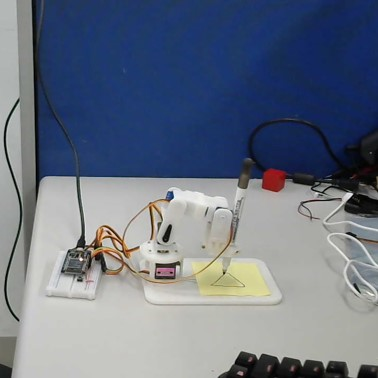
\includegraphics[width=0.4\linewidth]{figures/triangle_1.jpg}}
    ~    
    \subcaptionbox
        {執行畫星形指令
        \label{fig:fig-dataset-contrast-after-adjustment}}
        {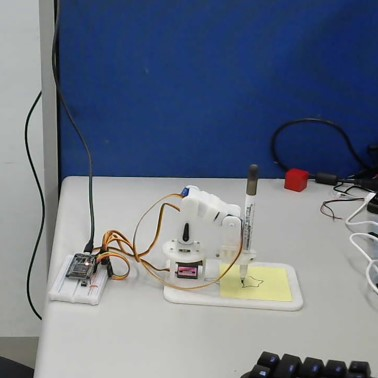
\includegraphics[width=0.4\linewidth]{figures/star_0.jpg}}
    ~
    \subcaptionbox
        {完成畫星形指令
        \label{fig:fig-dataset-contrast-after-adjustment}}
        {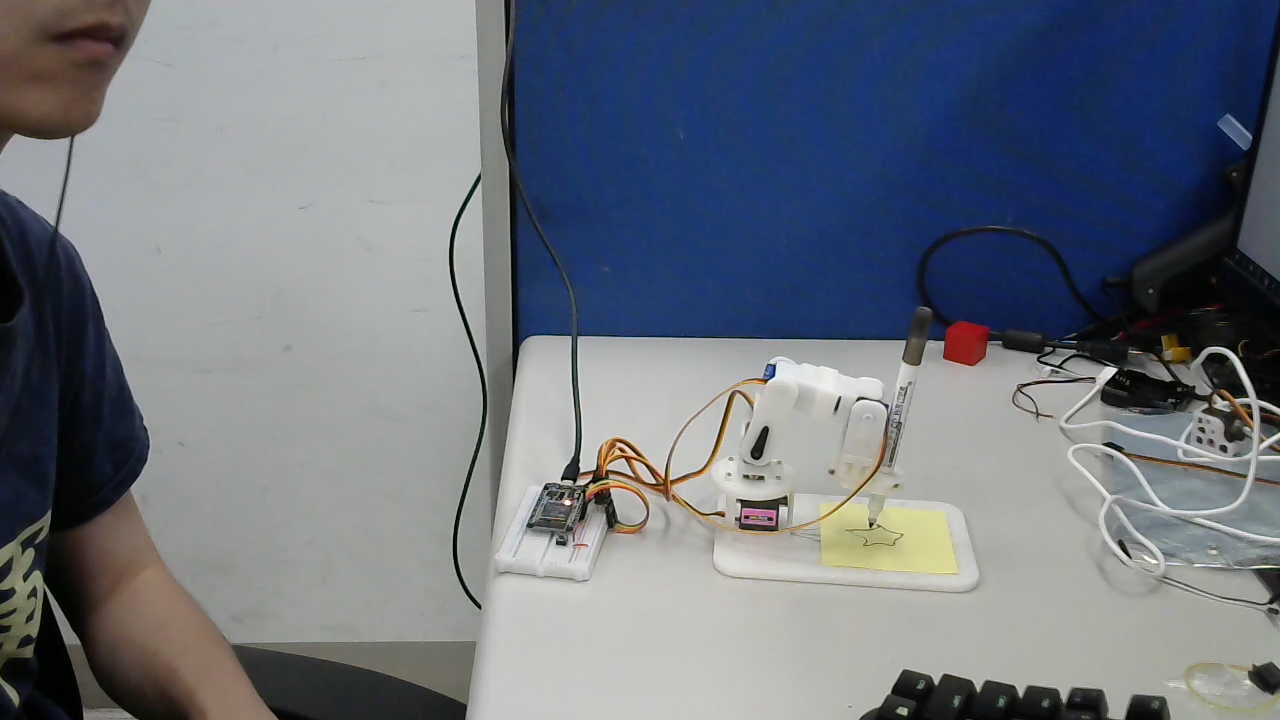
\includegraphics[width=0.4\linewidth]{figures/star_1.jpg}}   
\caption{實驗二:實驗過程縮圖}
\end{figure}

\section{實驗三:機械臂在自動運輸車上的應用}
\subsection{機械結構設計圖}
本實驗將機械臂與自動運輸車、鏡頭等硬體結合,設計了一台裝載機械臂的無人搬運車,以下為此硬體的詳細設計圖紙:
\begin{figure}[htbp]
    \centering
    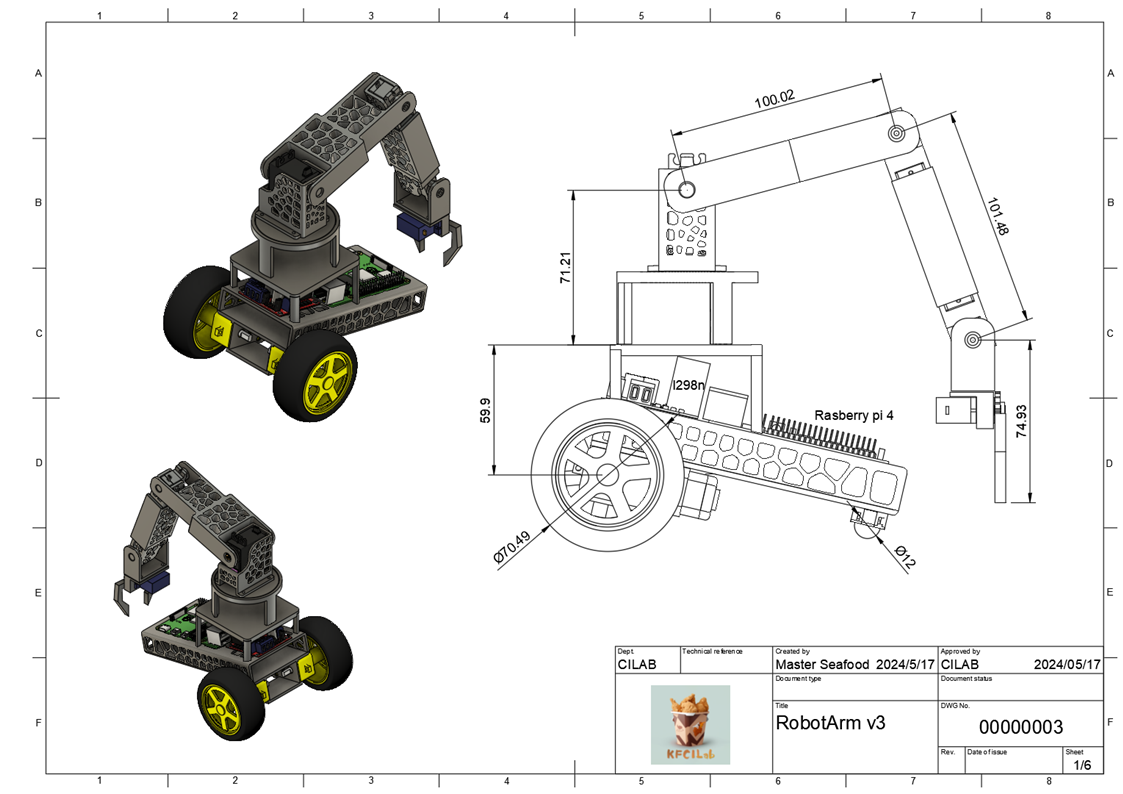
\includegraphics[width=0.9\textwidth]{figures/Armv3 (1).PNG}
    \caption{實驗三:設計圖紙 第一頁(單位:mm)}
    %\label{fig:Armv1Drawing_p1}}
\end{figure}

\begin{figure}[htbp]
    \centering
    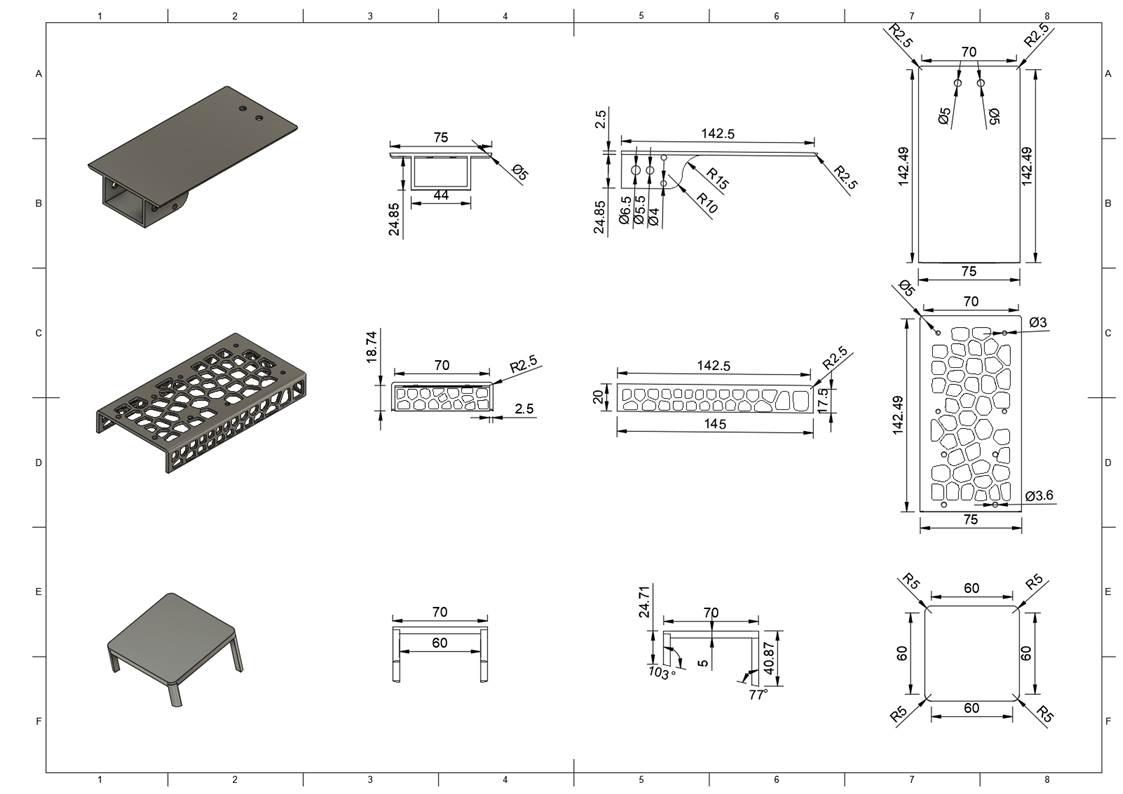
\includegraphics[width=0.9\textwidth]{figures/Armv3 (2).PNG}
    \caption{實驗三:設計圖紙 第二頁(單位:mm)}
\end{figure}

\begin{figure}[htbp]
    \centering
    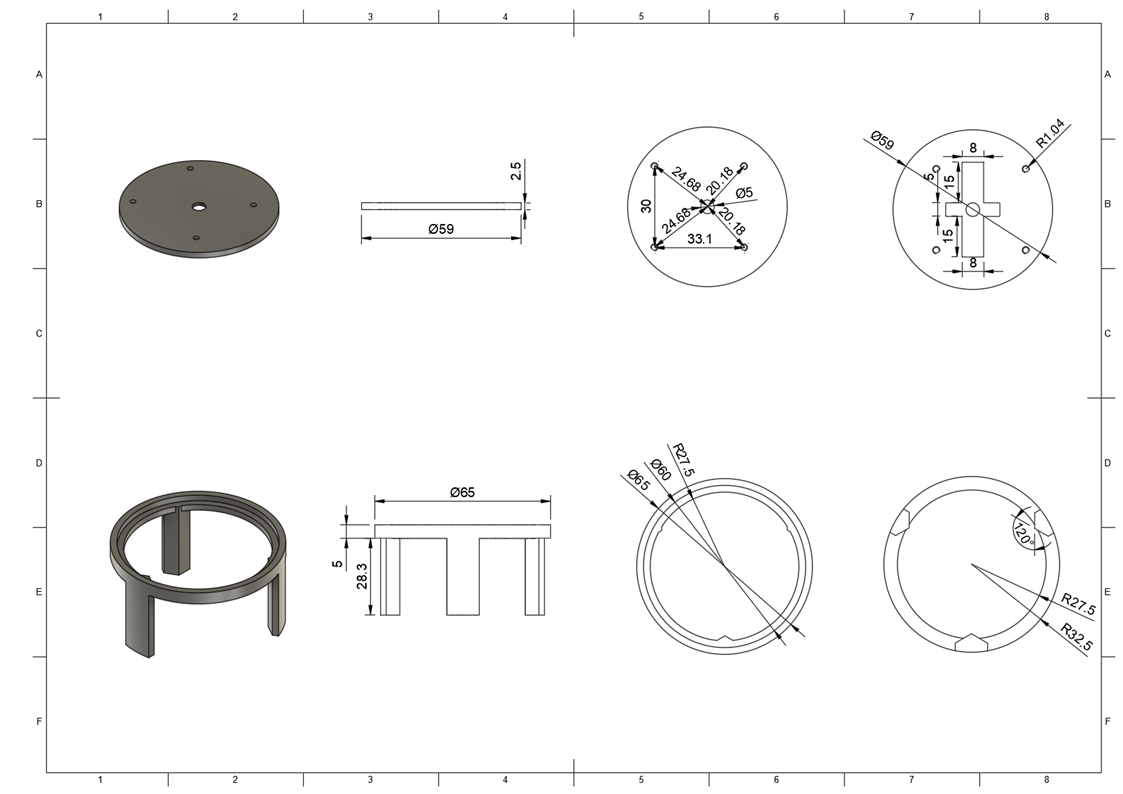
\includegraphics[width=0.9\textwidth]{figures/Armv3 (3).PNG}
    \caption{實驗三:設計圖紙 第三頁(單位:mm)}
\end{figure}

\begin{figure}[htbp]
    \centering
    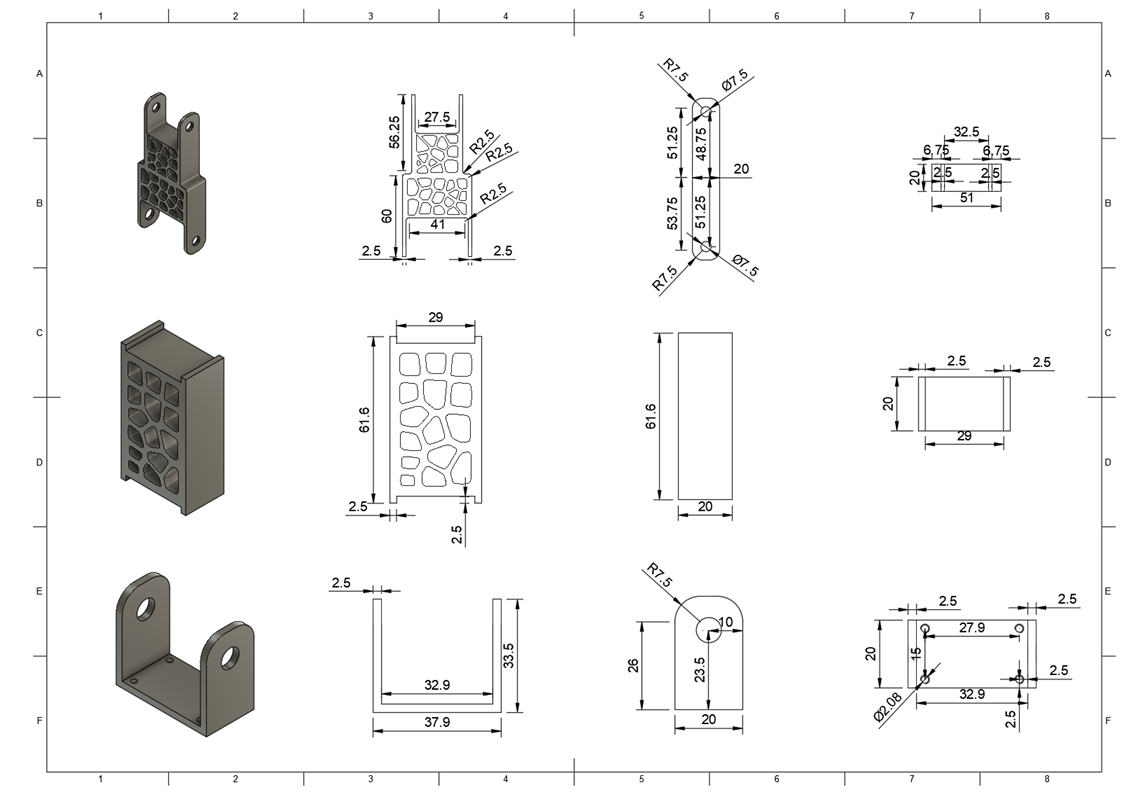
\includegraphics[width=0.9\textwidth]{figures/Armv3 (4).PNG}
    \caption{實驗三:設計圖紙 第四頁(單位:mm)}
\end{figure}

\begin{figure}[htbp]
    \centering
    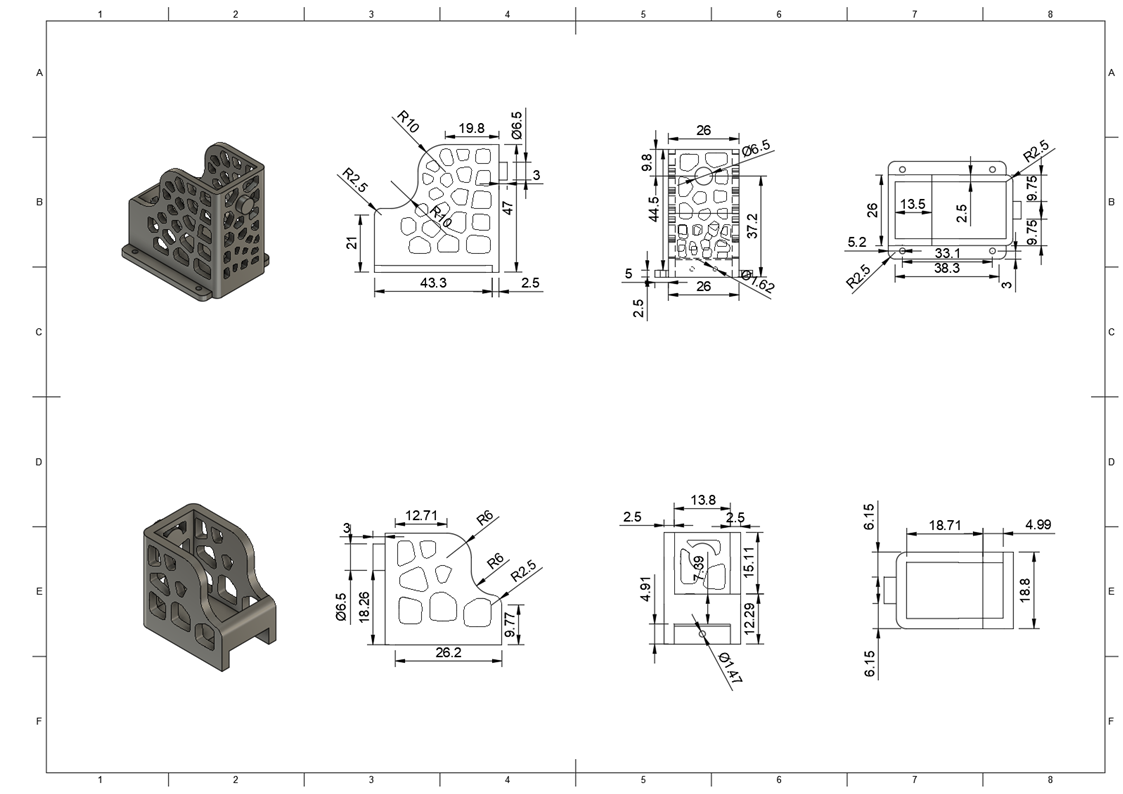
\includegraphics[width=0.9\textwidth]{figures/Armv3 (5).PNG}
    \caption{實驗三:設計圖紙 第五頁(單位:mm)}
\end{figure}

\begin{figure}[htbp]
    \centering
    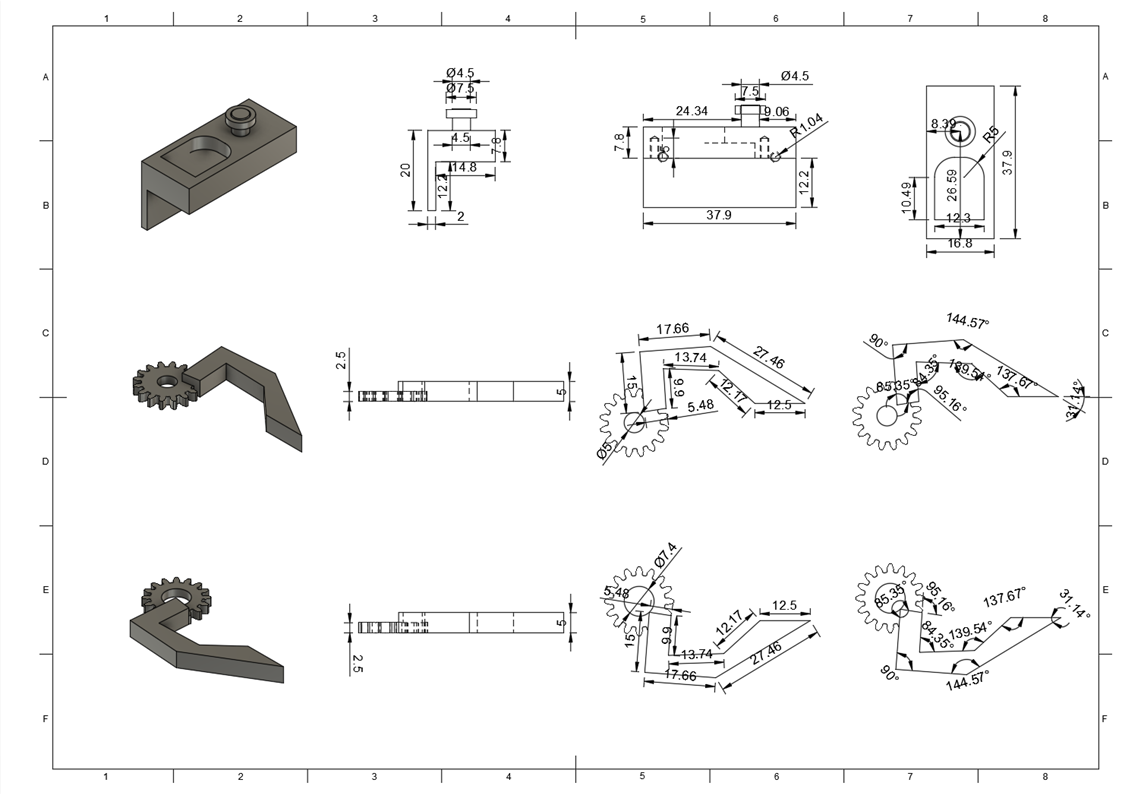
\includegraphics[width=0.9\textwidth]{figures/Armv3 (6).PNG}
    \caption{實驗三:設計圖紙 第六頁(單位:mm)}
\end{figure}

\subsection{函數設計}
在前兩個實驗的基礎上,我們進一步改進了控制流程,將機械臂與自動運輸車整合在一起。
這次,我們將控制函式進行細分,並模組化,使得大型語言模型能夠通過簡單的指令來控制機械臂和車輛的行動。
這種模組化的設計不僅降低了指令的複雜度,還減少了資源利用。
最終,我們能夠通過簡單的模組化指令來控制整個系統,
使得機械臂和車輛能夠協同工作,完成更複雜的任務。

\begin{itemize}
    \item find(color): 配合相機定位,驅動輪子尋找動應顏色的方塊。

    \item aim(color): 配合相機定位,驅動機械臂瞄準對應顏色的方塊。

    \item grab(): 驅動機械臂,抓取正下方的物品。

    \item reset(): 驅動機械臂,回到初始位置
\end{itemize}

\newpage
\subsection{下達指令的格式範例}
以下為指令格式:
\begin{listing}[h]
    \begin{minted}[frame=single,
                   framesep=3mm,
                   linenos=true,
                   xleftmargin=21pt,
                   tabsize=4]{js}
    {     
        role: "user",
        content : 
        "The following functions are available:\
        \
        find(color): Let the robot look for a block of a specific color.\
        color option: red, blue.\
        aim(color): Let the robot aim at a block of a specific color.\
        color option: red, blue\
        grab: Make the robot arm grab the block and put it down.\
        reset: Return the robotic arm to its initial position\
        (needs to be executed before each aiming).\
        \
        Please help me use the above functions to control the robot arm,\
        and do not output other text other than the above functions.\
        (Use "," to separate each step)"
    },
    {
        role: "user", 
        content: "Task: Please grab the red block, and then grab the blue block."
    }
    \end{minted}
\caption{實驗三:指令格式範例} 
\end{listing}

\begin{listing}[h]
    \begin{minted}[frame=single,
                   framesep=3mm,
                   linenos=true,
                   xleftmargin=21pt,
                   tabsize=4]{js}

    {
        role="assistant",
        content="find(red), aim(red), grab(), reset(), find(blue), aim(blue), grab()"
    }

    \end{minted}
\caption{實驗三:回傳格式範例} 
\end{listing}

\subsection{實驗結果}
以下為本實驗的實驗過程縮圖與總結:\\


\begin{table}[h]
    \centering
    \caption{實驗結果:Please grab the red block, and then grab the blue block.}
    \begin{tabular}{ccccc}
    \hline
    大型語言模型 & 總次數 & 成功次數 & 失敗次數 & 成功率 \\
    \hline
    GPT-4o & 10 & 9 & 1 & 0.9\\
    \hline
    GPT-3.5 Turbo & 10 & 7 & 3 & 0.7\\
    \hline
    \end{tabular}
\end{table}
在本次實驗中,我們增加了車輪、鏡頭等更多的硬體連動設備。由於每個任務都需要協調各個硬體的運作才能順利完成,我們在撰寫控制程式時,將各個重要指令整理成更加簡化且直觀的獨立函式,這樣可以方便大型語言模型在生成控制指令時直接呼叫這些函式。實驗結果顯示,這種方法取得了非常好的成效,顯著提高了控制指令的生成效率和準確性。然而,由於連動的硬體較多,在呼叫控制函式時難免會發生一些機械性的失誤。例如,鏡頭失真可能導致機械臂瞄準失誤,而車輪的移動則可能導致機械臂在夾取物體時出現掉落的情況。針對這些問題,我們希望在未來進一步優化硬體間的協調機制,以提升系統的穩定性和精確度。

\newpage
\begin{figure}[h]
    \centering
    \subcaptionbox
        {瞄準紅色方塊
        \label{fig:fig-dataset-contrast-after-adjustment}}
        {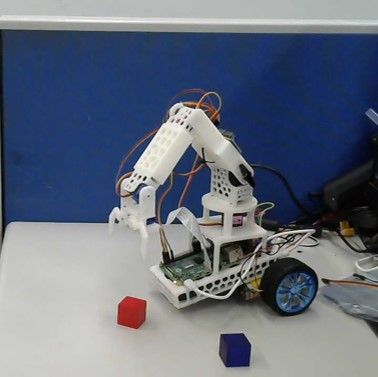
\includegraphics[width=0.4\linewidth]{figures/Exp3 (2)_square.jpg}}
    ~    
    \subcaptionbox
        {夾取紅色方塊
        \label{fig:fig-dataset-contrast-after-adjustment}}
        {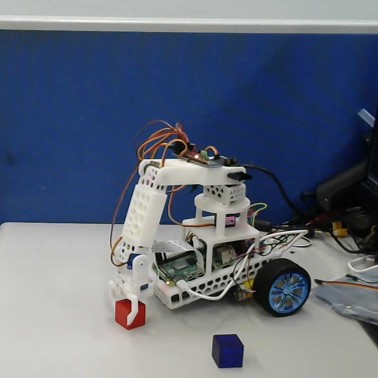
\includegraphics[width=0.4\linewidth]{figures/Exp3 (3)_square.jpg}}
    ~
    \subcaptionbox
        {夾取成功
        \label{fig:fig-dataset-contrast-after-adjustment}}
        {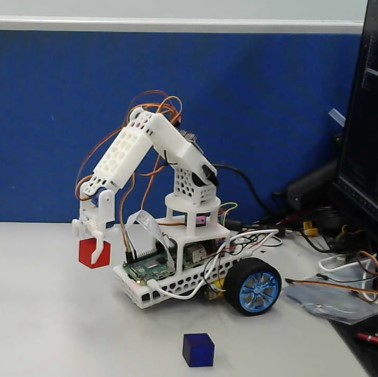
\includegraphics[width=0.4\linewidth]{figures/Exp3 (4)_square.jpg}}
    ~
    \subcaptionbox
        {瞄準藍色方塊
        \label{fig:fig-dataset-contrast-after-adjustment}}
        {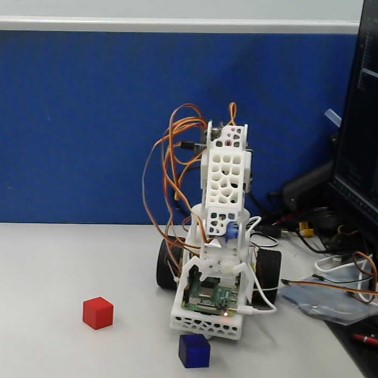
\includegraphics[width=0.4\linewidth]{figures/Exp3 (5)_square.jpg}}
    ~    
    \subcaptionbox
        {夾取藍色方塊
        \label{fig:fig-dataset-contrast-after-adjustment}}
        {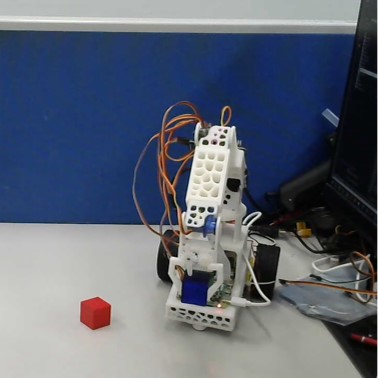
\includegraphics[width=0.4\linewidth]{figures/Exp3 (6)_square.jpg}}
    ~
    \subcaptionbox
        {夾取成功
        \label{fig:fig-dataset-contrast-after-adjustment}}
        {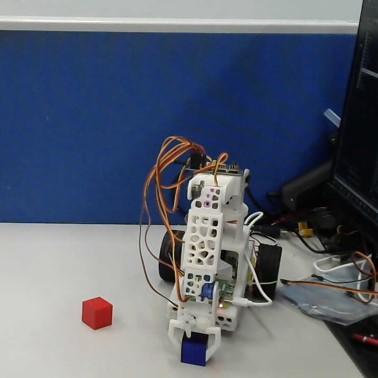
\includegraphics[width=0.4\linewidth]{figures/Exp3 (7)_square.jpg}}   
\caption{實驗三:實驗過程縮圖}
\end{figure}

\end{document}